\documentclass[12pt,letterpaper]{hmcpset}
\usepackage[margin=1in]{geometry}
\usepackage{graphicx}
\usepackage{esint}

% info for header block in upper right hand corner
\name{Box number: \underline{\hspace{1cm}} (name on back) }
\class{Math 60: Section \underline{\hspace{1cm}}}
\assignment{Assignment 6}
\duedate{Due Date: 10/19/18}

\begin{document}

\problemlist{
Section 6.1: 2, 9, 21, 31, 34, 40\\
Section 6.2: 13, 15\\
Section 7.2: 6, 14, 22, 28\\
Section 7.3: 4, 6
}

\begin{problem}
Section 6.1 \#2. In Exercises 2-7, calculate $\int_{\mathbf{x}} f \,ds$ where $f$ and $\mathbf{x}$ are as indicated.
$$ f(x, y, z) = xyz, \mathbf{x}(t) = (t, 2t, 3t), 0 \leq t \leq 2 $$
\end{problem}

\newpage

\begin{problem}
Section 6.1 \#9. In Exercises 8-16, calculate $\int_{\mathbf{x}} \mathbf{F} \cdot \,d\mathbf{s}$ where the vector field $\mathbf{F}$ and the path $\mathbf{x}$ are given.
$$ \mathbf{F} = (y+2) \mathbf{i} + x \mathbf{j}, \mathbf{x}(t) = (\sin{t}, -\cos{t}), 0 \leq t \leq \frac{\pi}{2} $$
\end{problem}

\newpage

\begin{problem}
Section 6.1 \#21. Let $\mathbf{F} = (x^2 + y) \mathbf{i} + (y - x) \mathbf{j}$ and consider the two paths
$$ \mathbf{x}(t) = (t, t^2), 0 \leq t \leq 1 \text{ and} $$
$$ \mathbf{y}(t) = (1 - 2t, 4t^2 - 4t + 1), 0 \leq t \leq \frac{1}{2}. $$
\begin{enumerate}
	\item[(a)] Calculate $\int_{\mathbf{x}} \mathbf{F} \cdot \,d\mathbf{s}$ and $\int_{\mathbf{y}} \mathbf{F} \cdot \,d\mathbf{s}$.
	\item[(b)] By considering the image curves of the paths $\mathbf{x}$ and $\mathbf{y}$, discuss your answers in part (a).
\end{enumerate}
\end{problem}

\newpage

\begin{problem}
Section 6.1 \#31. Evaluate $ \int_C yz \,dx - xz \,dy + xy \,dz $, where $C$ is the line segment from $(1, 1, 2)$ to $(5, 3, 1)$.
\end{problem}

\newpage

\begin{problem}
Section 6.1 \#34. Tom Sawyer is whitewashing a picket fence. The bases of the fenceposts are arranged in the $xy$-plane as the quarter circle $x^2 + y^2 = 25, x, y \geq 0$, and the height of the fencepost at point $(x, y)$ is given by $h(x, y) = 10 - x - y$ (units are feet). Use a scalar line integral to find the area of one side of the fence. (See Figure 6.16.)\\
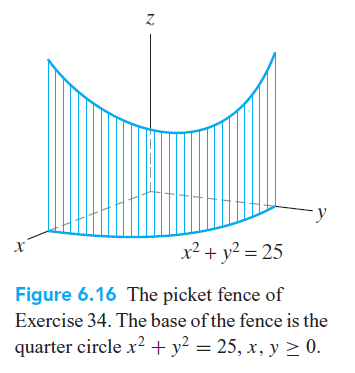
\includegraphics[width=0.5\textwidth]{figure6-16.png}
\end{problem}

\newpage

\begin{problem}
Section 6.1 \#40. You are traveling through Cleveland, famous for its lake-effect snow in winter that makes driving quite treacherous. Suppose that you are currently located 20 miles due east of Cleveland and are attempting to drive to a point 20 miles due west of Cleveland. Further suppose that if you are $s$ miles from the center of Cleveland, where the weather is the worst, you can drive at a rate of at most $v(s) = 2s + 20$ miles per hour.
\begin{enumerate}
	\item[(a)] How long will the trip take if you drive on a straight-line path directly through Cleveland? (Assume that you always drive at the maximum speed possible.)
	\item[(b)] How long will the trip take if you avoid the middle of the city by driving along a semicircular path with Cleveland at the center? (Again, assume that you drive at the maximum speed possible.)
	\item[(a)] Repeat parts (a) and (b), this time using $v(s) = (s^2 / 16) + 25$ miles per hour as the maximum speed that you can drive.
\end{enumerate}
\end{problem}

\newpage

\begin{problem}
Section 6.2 \#13. Evaluate $\oint_C (x^4 y^5 - 2y) \,dx + (3x + x^5 y^4) \,dy$, where $C$ is the oriented curve pictured in Figure 6.29.\\
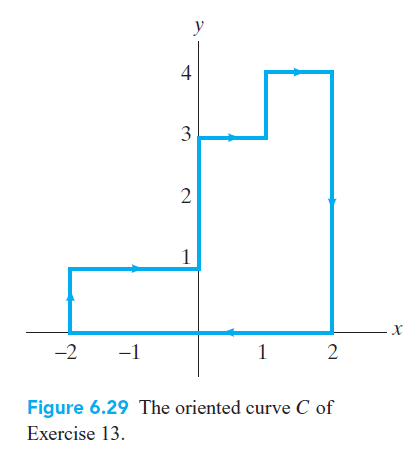
\includegraphics[width=0.5\textwidth]{figure6-29.png}
\end{problem}

\newpage

\begin{problem}
Section 6.2 \#15.
\begin{enumerate}
	\item[(a)] Sketch the curve given parametrically by $\mathbf{x}(t) = (1 - t^2, t^3 - t)$
	\item[(b)] Find the area inside the closed loop of the curve.
\end{enumerate}
\end{problem}

\newpage

\begin{problem}
Section 7.2 \#6. Find $ \iint_S (x^2 + y^2) \,dS $, where $S$ is the lateral surface of the cylinder of radius $a$ and height $h$ whose axis is the $z$-axis.
\end{problem}

\newpage

\begin{problem}
Section 7.2 \#14. In Exercises 10-18, let $S$ denote the closed cylinder with bottom given by $z = 0$, top given by $z = 4$, and lateral surface given by the equation $x^2 + y^2 = 9$. Orient $S$ with outward normals. Determine the indicated scalar and vector surface integrals.
$$ \iint_S (x \mathbf{i} + y \mathbf{j}) \cdot \,d \mathbf{S}$$
\end{problem}

\newpage

\begin{problem}
Section 7.2 \#22. In Exercises 19-22, find the flux of the given vector field $\mathbf{F}$ across the upper hemisphere $ x^2 + y^2 + z^2 = a^2, z \geq 0$. Orient the hemisphere with an upward-pointing normal.
$$ \mathbf{F} = x^2 \mathbf{i} + xy \mathbf{j} + xz \mathbf{k} $$
\end{problem}

\newpage

\begin{problem}
Section 7.2 \#28. The glass dome of a futuristic greenhouse is shaped like the surface $ z = 8 - 2x^2 - 2y^2 $. The greenhouse has a flat dirt floor at $z = 0$. Suppose that the temperature $T$, at points in and around the greenhouse, varies as
$$ T(x, y, z) = x^2 + y^2 + 3(z-2)^2. $$
Then the temperature gives rise to a \textbf{heat flux density field $\mathbf{H}$} given by $\mathbf{H} = -k \nabla T$. (Here $k$ is a positive constant that depends on the insulating properties of the particular medium.) Find the total heat flux outward across the dome and the surface of the ground if $k = 1$ on the glass and $k = 3$ on the ground.
\end{problem}

\newpage

\begin{problem}
Section 7.3 \#4. In Exercises 1-4, verify Stokes's Theorem for the given surface and vector field.
\begin{center}
$S$ is defined by $x^2 + y^2 + z^2 = 4, z \leq 0$, oriented by downward normal;
\end{center}
$$ \mathbf{F} = (2y - z) \mathbf{i} + (x + y^2 - z) \mathbf{j} + (4y - 3x) \mathbf {k}. $$
\end{problem}

\newpage

\begin{problem}
Section 7.3 \#6. In Exercises 6-9, verify Gauss's theorem for the given three-dimensional region $D$ and vector field $\mathbf{F}$.
$$ \mathbf{F} = x \mathbf{i} + y \mathbf {j} + z \mathbf {k}, $$
$$ D = \{ (x, y, z) | 0 \leq z \leq 9 - x^2 - y^2 \} $$
\end{problem}
\end{document}
